%% CV_yunjaeCho_nota.tex — Yunjae Cho
%% Nota AI — [NetsPresso] Physical AI Engineer Intern (id 233322) 지원용
%% Compile: pdflatex CV_yunjaeCho_nota.tex
\documentclass[10pt,a4paper]{article}

\usepackage[T1]{fontenc}
\usepackage[utf8]{inputenc}
\usepackage{times}
\usepackage[scaled=0.92]{helvet}
\renewcommand{\ttdefault}{cmtt}
\usepackage[margin=0.65in]{geometry}
\usepackage{xcolor}
\usepackage{tabularx}
\usepackage{array}
\usepackage{graphicx}
\usepackage[hidelinks]{hyperref}

% ---- Colors ----
\definecolor{accent}{RGB}{215,80,50}
\definecolor{darkgray}{RGB}{60,60,60}

% ---- Custom section ----
\makeatletter
\renewcommand{\section}[1]{%
  \par\vspace{10pt}%
  {\color{accent}\Large\bfseries #1}%
  \par\vspace{-6pt}%
  {\color{accent}\rule{\textwidth}{0.8pt}}%
  \par\vspace{4pt}%
  \@afterheading}
\makeatother

% ---- Entry macro ----
\newcommand{\cvEntry}[4]{%
  \par\vspace{3pt}%
  \noindent\begin{tabularx}{\textwidth}{@{}X r@{}}
    \textbf{#1} & {\color{accent}#2} \\
  \end{tabularx}\par\vspace{-4pt}%
  \noindent\begin{tabularx}{\textwidth}{@{}X r@{}}
    \textit{#3} & {\color{accent}\textit{#4}} \\
  \end{tabularx}\par}

% ---- Single-line entry ----
\newcommand{\cvLine}[2]{%
  \par\vspace{2pt}%
  \noindent\begin{tabularx}{\textwidth}{@{}X r@{}}
    \textbf{#1} & {\color{accent}#2} \\
  \end{tabularx}\par}

% ---- Compact bullet list ----
\newenvironment{cvitems}{%
  \vspace{-2pt}%
  \begin{list}{\textbullet}{%
    \setlength{\leftmargin}{1.4em}%
    \setlength{\rightmargin}{0em}%
    \setlength{\topsep}{1pt}%
    \setlength{\itemsep}{2pt}%
    \setlength{\parsep}{0pt}%
    \setlength{\labelsep}{0.6em}}%
}{\end{list}\vspace{2pt}}

\pagenumbering{gobble}
\setlength{\parindent}{0pt}
\setlength{\parskip}{0pt}

\begin{document}

% ================= HEADER =================
\noindent
\begin{minipage}[c]{0.16\textwidth}
  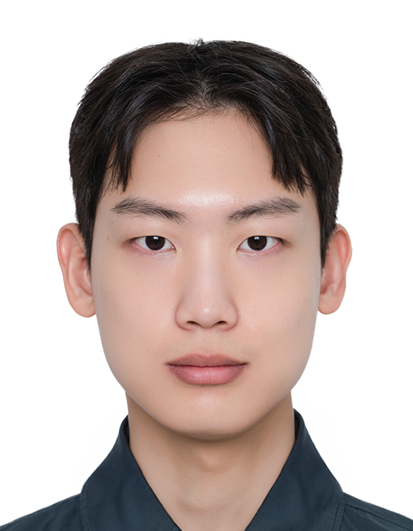
\includegraphics[width=\linewidth]{photo.jpg}
\end{minipage}%
\hfill%
\begin{minipage}[c]{0.82\textwidth}
  \raggedright
  {\fontsize{28}{32}\selectfont Yunjae \textbf{Cho}}\\[6pt]
  {\color{darkgray}\small
    Phone: 010-2664-6276 \quad{\color{accent}$\bullet$}\quad
    Email: \href{mailto:devilishvoice@inha.edu}{devilishvoice@inha.edu} \quad{\color{accent}$\bullet$}\quad
    GitHub: \href{https://github.com/hashbraun}{github.com/hashbraun} \quad{\color{accent}$\bullet$}\quad
    Portfolio: \href{https://hashbraun.github.io/portfolio.html}{hashbraun.github.io/portfolio.html}
  }
\end{minipage}

\vspace{6pt}

% ================= PROFILE =================
\noindent{\color{darkgray}\small
Undergraduate AI engineer building CV/VLA systems on real hardware --- \textbf{SO-101 teleop}, \textbf{TensorRT-deployed detectors}, \textbf{Cosmos-based world models}.\\
I learn by building: reviewing new papers weekly (ICLR 2026 X-VLA, NVIDIA Cosmos 3) and porting the ideas into the next project.\\
Results are reported without embellishment; fallback paths are placed \emph{inside} the system itself --- Recovery FSM in a 6-DOF arm, 5-runtime export in a production detector.\\
Focus: VLA on SO-101, action-conditioned World Models, on-device optimization (TensorRT / ONNX / OpenVINO, INT8 in progress).
}

% ==================== EDUCATION ====================
\section{Education}
\cvEntry{Inha University}{Incheon, Korea}{B.S.\ in Artificial Intelligence Engineering \quad {\small GPA: 3.59 / 4.5}}{Mar. 2021 -- Feb. 2027 (Expected)}

% ==================== RESEARCH INTERESTS ====================
\section{Research Interests}
{\color{accent}$\bullet$}\; \textbf{Vision-Language-Action (VLA)} \; {\color{accent}$\bullet$}\; \textbf{World-Action Model (WAM)} \; {\color{accent}$\bullet$}\; \textbf{On-Device Model Optimization} \; {\color{accent}$\bullet$}\; \textbf{Data-efficient Learning}

% ==================== RESEARCH EXPERIENCE ====================
\section{Research Experience}

\cvEntry{HDC LABS (AI LAB)}{Seoul, Korea}{AI Researcher}{Mar. 2026 -- Present}
\begin{cvitems}
  \item Contributed to multiple in-house pipelines including a \textbf{semi-auto labeling tool}, a \textbf{TTS dataset construction pipeline}, and internal \textbf{data \& model monitoring / validation systems} (see Projects).
  \item Presented at \textbf{AI Lab Weekly Paper Reviews} on recent VLA and World Model papers, including \textbf{X-VLA} (ICLR 2026) and \textbf{NVIDIA Cosmos 3} --- covering architecture, training, and experiments (see Talks).
\end{cvitems}

\vspace{4pt}
\cvEntry{RILS Lab, Inha University}{Incheon, Korea}{Undergraduate Researcher \quad {\small (Advised by Prof.\ Woojin Ahn)}}{Jul. 2025 -- Mar. 2026}
\begin{cvitems}
  \item Built \textbf{end-to-end experience in VLA learning pipelines} on \textbf{SO-101} bi-manipulator hardware --- from teleop data collection to policy training and closed-loop evaluation.
  \item Participated in \textbf{weekly seminars} and the \textbf{Physical AI Hackathon}.
\end{cvitems}

% ==================== PROJECTS ====================
\section{Selected Projects}

% ---------- 1. VLA Bi-manipulator (SO-101) ----------
\cvEntry{VLA Imitation Learning Bi-manipulator (SO-101)}{}{Researcher \quad {\small @ RILS Lab}}{Jul. 2025 -- Feb. 2026}
\begin{cvitems}
  \item Developed a bi-manipulator VLA policy that mitigates \textbf{location memorization} and \textbf{pose hallucination} common in RGB-only imitation policies.
  \item Set up the \textbf{teleoperation rig}, ran on-robot \textbf{SO-101 demonstration collection}, and handled episode curation, policy training, and closed-loop evaluation.
  \item Fused features from three camera streams (top / front / wrist) with proprioceptive state, incorporating frame--action temporal context to improve motion direction and velocity estimation.
  \item Reported real-hardware rollout success rate at \textbf{20--30\% (2--3/10)}, without embellishment, to drive the next data-collection iteration toward under-covered failure modes.
\end{cvitems}

% ---------- 2. World Model — INHA Challenge (Cosmos) ----------
\cvEntry{Action-Conditioned Video Generation World Model --- 2026 INHA AI Challenge}{}{Individual Entry}{Jul. 2026 -- Aug. 2026}
\begin{cvitems}
  \item Built an \textbf{action-conditioned video generation world model} predicting a robot's future frames from the first frame and a joint-action sequence.
  \item Added an action-injection module (trained at base LR) to route SO-100 action tokens into the video backbone, unlocking Cosmos-Predict3-Nano (\textbf{action MAE $-43.2\%$}).
  \item Fine-tuned Cosmos-Predict3-Nano with \textbf{LoRA (rank 32)} on attention and MLP projections for action--video mapping (\textbf{action MAE $-8.6\%$}).
  \item Identified an action-space mismatch with the Cosmos3 pretraining distribution and redesigned the representation using end-effector deltas and normalized gripper states, further reducing action MAE by \textbf{8.5\%}.
\end{cvitems}

% ---------- 3. 6-DOF Path Replanning ----------
\cvEntry{Dynamic Obstacle-Aware Path Replanning for a 6-DOF Robot Arm}{}{Team Member \quad {\small (3-person team)}}{Aug. 2025 -- Dec. 2025}
\begin{cvitems}
  \item Implemented \textbf{collision-aware grasping} for warehouse picking where dynamic obstacles enter the planned trajectory mid-execution.
  \item Built a UR5e perception pipeline (RGB-D RealSense, point-cloud generation, probabilistic \textbf{OctoMap} mapping, 10 Hz MoveIt2 planning-scene updates) with YOLO-based detection and ICP-refined pose estimation.
  \item Designed a MoveIt2 motion pipeline using \textbf{RRT-Connect} (OMPL) with FCL continuous collision checking for trajectory-level future collision prediction.
  \item End-to-end \textbf{Recovery FSM} (Detect $\to$ Stop $\to$ Replan $\to$ Resume) placed the fallback path \textit{inside} the system, verified reactive replanning on Gazebo with a \textbf{60\% (3/5)} success rate.
\end{cvitems}

% ---------- 4. Safety Detection + TensorRT Deployment ----------
\cvEntry{Construction-Safety Detection + TensorRT Deployment --- w/ HDC LABS}{}{AI Researcher}{Jun. 2026 -- Aug. 2026}
\begin{cvitems}
  \item Diagnosed val--field metric divergence on a 10-class construction-site detector; re-established a scene-level held-out split and rebalanced under-represented classes.
  \item Deployed a \textbf{7-model WBF ensemble} in production; recovered pump-car \textbf{F1 0.00 $\to$ 0.57} on the deployed v1.
  \item Deployed via \textbf{TensorRT FP16}: \textbf{3.9$\times$ speedup} with mAP@0.5 \textbf{0.6317 $\to$ 0.6265} (retention \textbf{99.18\%}).
  \item Extended to a 5-runtime export pipeline (PyTorch / ONNX / TensorRT FP16 / OpenVINO); INT8 quantization build in progress.
\end{cvitems}

% ---------- Others (compact) ----------
\vspace{2pt}
\textbf{Others}
\begin{cvitems}
  \item \textbf{Smart-Elevator Semi-Auto Labeling Tool} --- YOLO11m-seg (\textbf{mAP@0.5 = 0.978}) + SAM2 polygon-mask prompting; 60-frame clip labeling \textbf{30 min $\to$ 4 min ($\approx$7.5$\times$)}, multi-user web tool in production (w/ Hyundai Elevator).
  \item \textbf{On-Device Personal Memory Agent} --- Corrective-RAG + Reflection dual-loop, BM25+dense hybrid with RRF and cross-encoder rerank; Hit@1 \textbf{+6\%p}, Recall@3 \textbf{+10\%p} on a 30-query bench.
  \item \textbf{CV AI Agent: VLM Video Action Recognition} --- Qwen3-VL structured-output pipeline with prompt constraints and adaptive ffmpeg downsampling; full-dataset batch on SLURM without training.
  \item \textbf{AGI Auto-labeling Pipeline} (w/ Korea Institute of Robotics, KIRO) --- SAM3 + GPT-4o-mini with DBSCAN mask merging for the unknown-object problem.
  \item Prior projects: Crack Detection (SegFormer + Skeleton), Seq2Seq NMT, LoRA fine-tuning, ControlNet colorization, time-series anomaly detection.
\end{cvitems}

% ==================== TALKS / PAPER REVIEWS ====================
\section{Talks \& Paper Reviews}

\noindent{\color{darkgray}\small
Presenter at HDC LABS AI Lab Weekly Paper Reviews. I unpack a new paper (architecture, training, experiments) in the seminar, then port the idea into the next project.
}
\vspace{4pt}

\cvEntry{Cosmos 3: Omnimodal World Models for Physical AI \small \href{https://hashbraun.github.io/seminar/seminar_cosmos_nano.html}{[slides]}}{NVIDIA (2026)}{HDC LABS AI Lab Weekly Paper Review}{Aug. 21, 2026}
\begin{cvitems}
  \item Covered WAM (World Action Model) with three modes (Forward / Inverse Dynamics / Policy) unified in a single \textbf{MoT dual-pathway}; 3-stage training (Pre-training $\to$ Action Mid-training $\to$ Specialist).
  \item Analyzed the finding that \textbf{action mid-training outweighs parameter scaling} (Table 18); ported the observation directly into 2026 INHA AI Challenge tuning with Cosmos-Predict3-Nano (sample 164, Action MAE 0.144).
\end{cvitems}

\vspace{4pt}
\cvEntry{X-VLA: Soft-Prompted Transformer as Scalable Cross-Embodiment VLA \small \href{https://hashbraun.github.io/seminar/X-VLA_ICLR2026_review.pdf}{[slides]}}{ICLR 2026}{HDC LABS AI Lab Weekly Paper Review}{Aug. 2026}
\begin{cvitems}
  \item Explained how cross-embodiment heterogeneity is absorbed via domain-specific \textbf{Soft Prompts} (0.04\% of all parameters) on a Florence-2 backbone with \textbf{Flow Matching} (OT-based velocity prediction).
  \item Analyzed the 2-step adaptation (prompt warm-up $\to$ joint training) and the result that \textbf{a 0.9B model outperforms 7--9B baselines} (OpenVLA / UniVLA / $\pi_0$) across six simulation benchmarks --- structural design outweighed scale.
\end{cvitems}

% ==================== AWARDS ====================
\section{Awards \& Honors}
\cvLine{Carbon Neutrality Innovation Academy, 5th Cohort --- \textit{1st Place} \small (AI Lead; on-device NPU-target safety-monitoring; YOLOv8m-seg mAP50 $\approx$ 0.90)}{Aug. 2025 -- Dec. 2025}
\cvLine{2026 INHA AI Challenge --- \textit{11th (Undergraduate)} of 215 (Individual Entry, score 0.24524, lower-better)}{Jul. 2026 -- Aug. 2026}
\cvLine{Service Scholarship --- Inha University \small (Student Association President)}{Mar. 2025 -- Dec. 2025}
\cvLine{Work-Study Scholarship --- Inha University \small (TA: Database, Computer Vision)}{Mar. 2025 -- Dec. 2025}

% ==================== EXTRACURRICULAR ====================
\section{Leadership \& Activities}
\begin{cvitems}
  \item \textbf{Student Association President}, Inha University AI Engineering --- scaled end-of-semester assembly \textbf{10 $\to$ 70+ attendees}, founded department student lounge (Mar. 2025 -- Dec. 2025).
  \item \textbf{13th i-STARTUP LAB} --- Team Leader / Presenter; context-aware collaboration tool (React, Firebase, ChatGPT API) (May 2025 -- Jul. 2025).
  \item \textbf{Google Developer Groups on Campus INHA} --- Core Member, BD Lead; planned a 16-day, 40-person hackathon; led DevSprint 2025 (3-week MVP program) with four teams end-to-end (Sep. 2024 -- Jul. 2025).
  \item \textbf{AWS Cloud Club INHA 3rd} --- backend contributor to Taggle (Sep. 2024 -- Dec. 2024).
\end{cvitems}

% ==================== TEACHING ====================
\section{Teaching}
\cvLine{Teaching Assistant --- Inha University (Database, Computer Vision)}{Mar. 2025 -- Dec. 2025}
\cvLine{Instructor --- Haesol Mathematics Academy (Middle-school math)}{Mar. 2025 -- Jul. 2025}

% ==================== SKILLS ====================
\section{Skills}
\noindent\begin{tabularx}{\textwidth}{@{}l X@{}}
\textbf{Robotics / Physical AI} & LeRobot, SO-101 teleop, ROS2 (Humble), MoveIt2 / RViz2, Gazebo, Isaac Sim, RRT-Connect (OMPL), FCL, OctoMap \\
\textbf{Model Optimization}     & TensorRT (FP16), ONNX, OpenVINO \quad {\small (INT8 quantization: in progress)} \\
\textbf{DL / VLA / WM}          & PyTorch, Hugging Face (Transformers, Diffusers, PEFT/LoRA), Cosmos-Predict3, Qwen3-VL, SAM2/3, YOLO11 \\
\textbf{Data / Retrieval}       & NumPy, Pandas, Matplotlib, LanceDB, BM25 (rank-bm25), Cross-encoder rerank \\
\textbf{Backend / Infra}        & FastAPI, MySQL, Firebase, Node.js, Docker, SLURM, Linux, Git, Conda, SSH, WSL2 \\
\textbf{Frontend}               & React, TypeScript, Figma \\
\textbf{Programming}            & Python, C++, Java \\
\end{tabularx}

% ==================== OTHERS ====================
\section{Others}
\textbf{English:} OPIc IM1 (Mar. 2026) \quad {\color{accent}$\bullet$}\quad \textbf{Certification:} SQLD (May 2025)

\end{document}
